\subsection{شبیه‌سازی کانال رول استند در حضور کنترل‌کننده LQDG}
در بخش
\label{roll_LQDG}
شبیه‌سازی کانال رول استند چهارپره انجام شد. در این بخش به بررسی عملکرد چهارپره در حضور کنترل‌کننده LQDG پرداخته می‌شود. کنترل‌کننده LQDG در بخش‌های
\ref{openloop_game}
و
\ref{closedloop_game}
بررسی شده است.
 در شبیه‌سازی برای بهینه‌سازی ضرایب وزنی از روش
TCACS \cite{Karimi2010}
استفاده شده است.
\begin{figure}[H]
	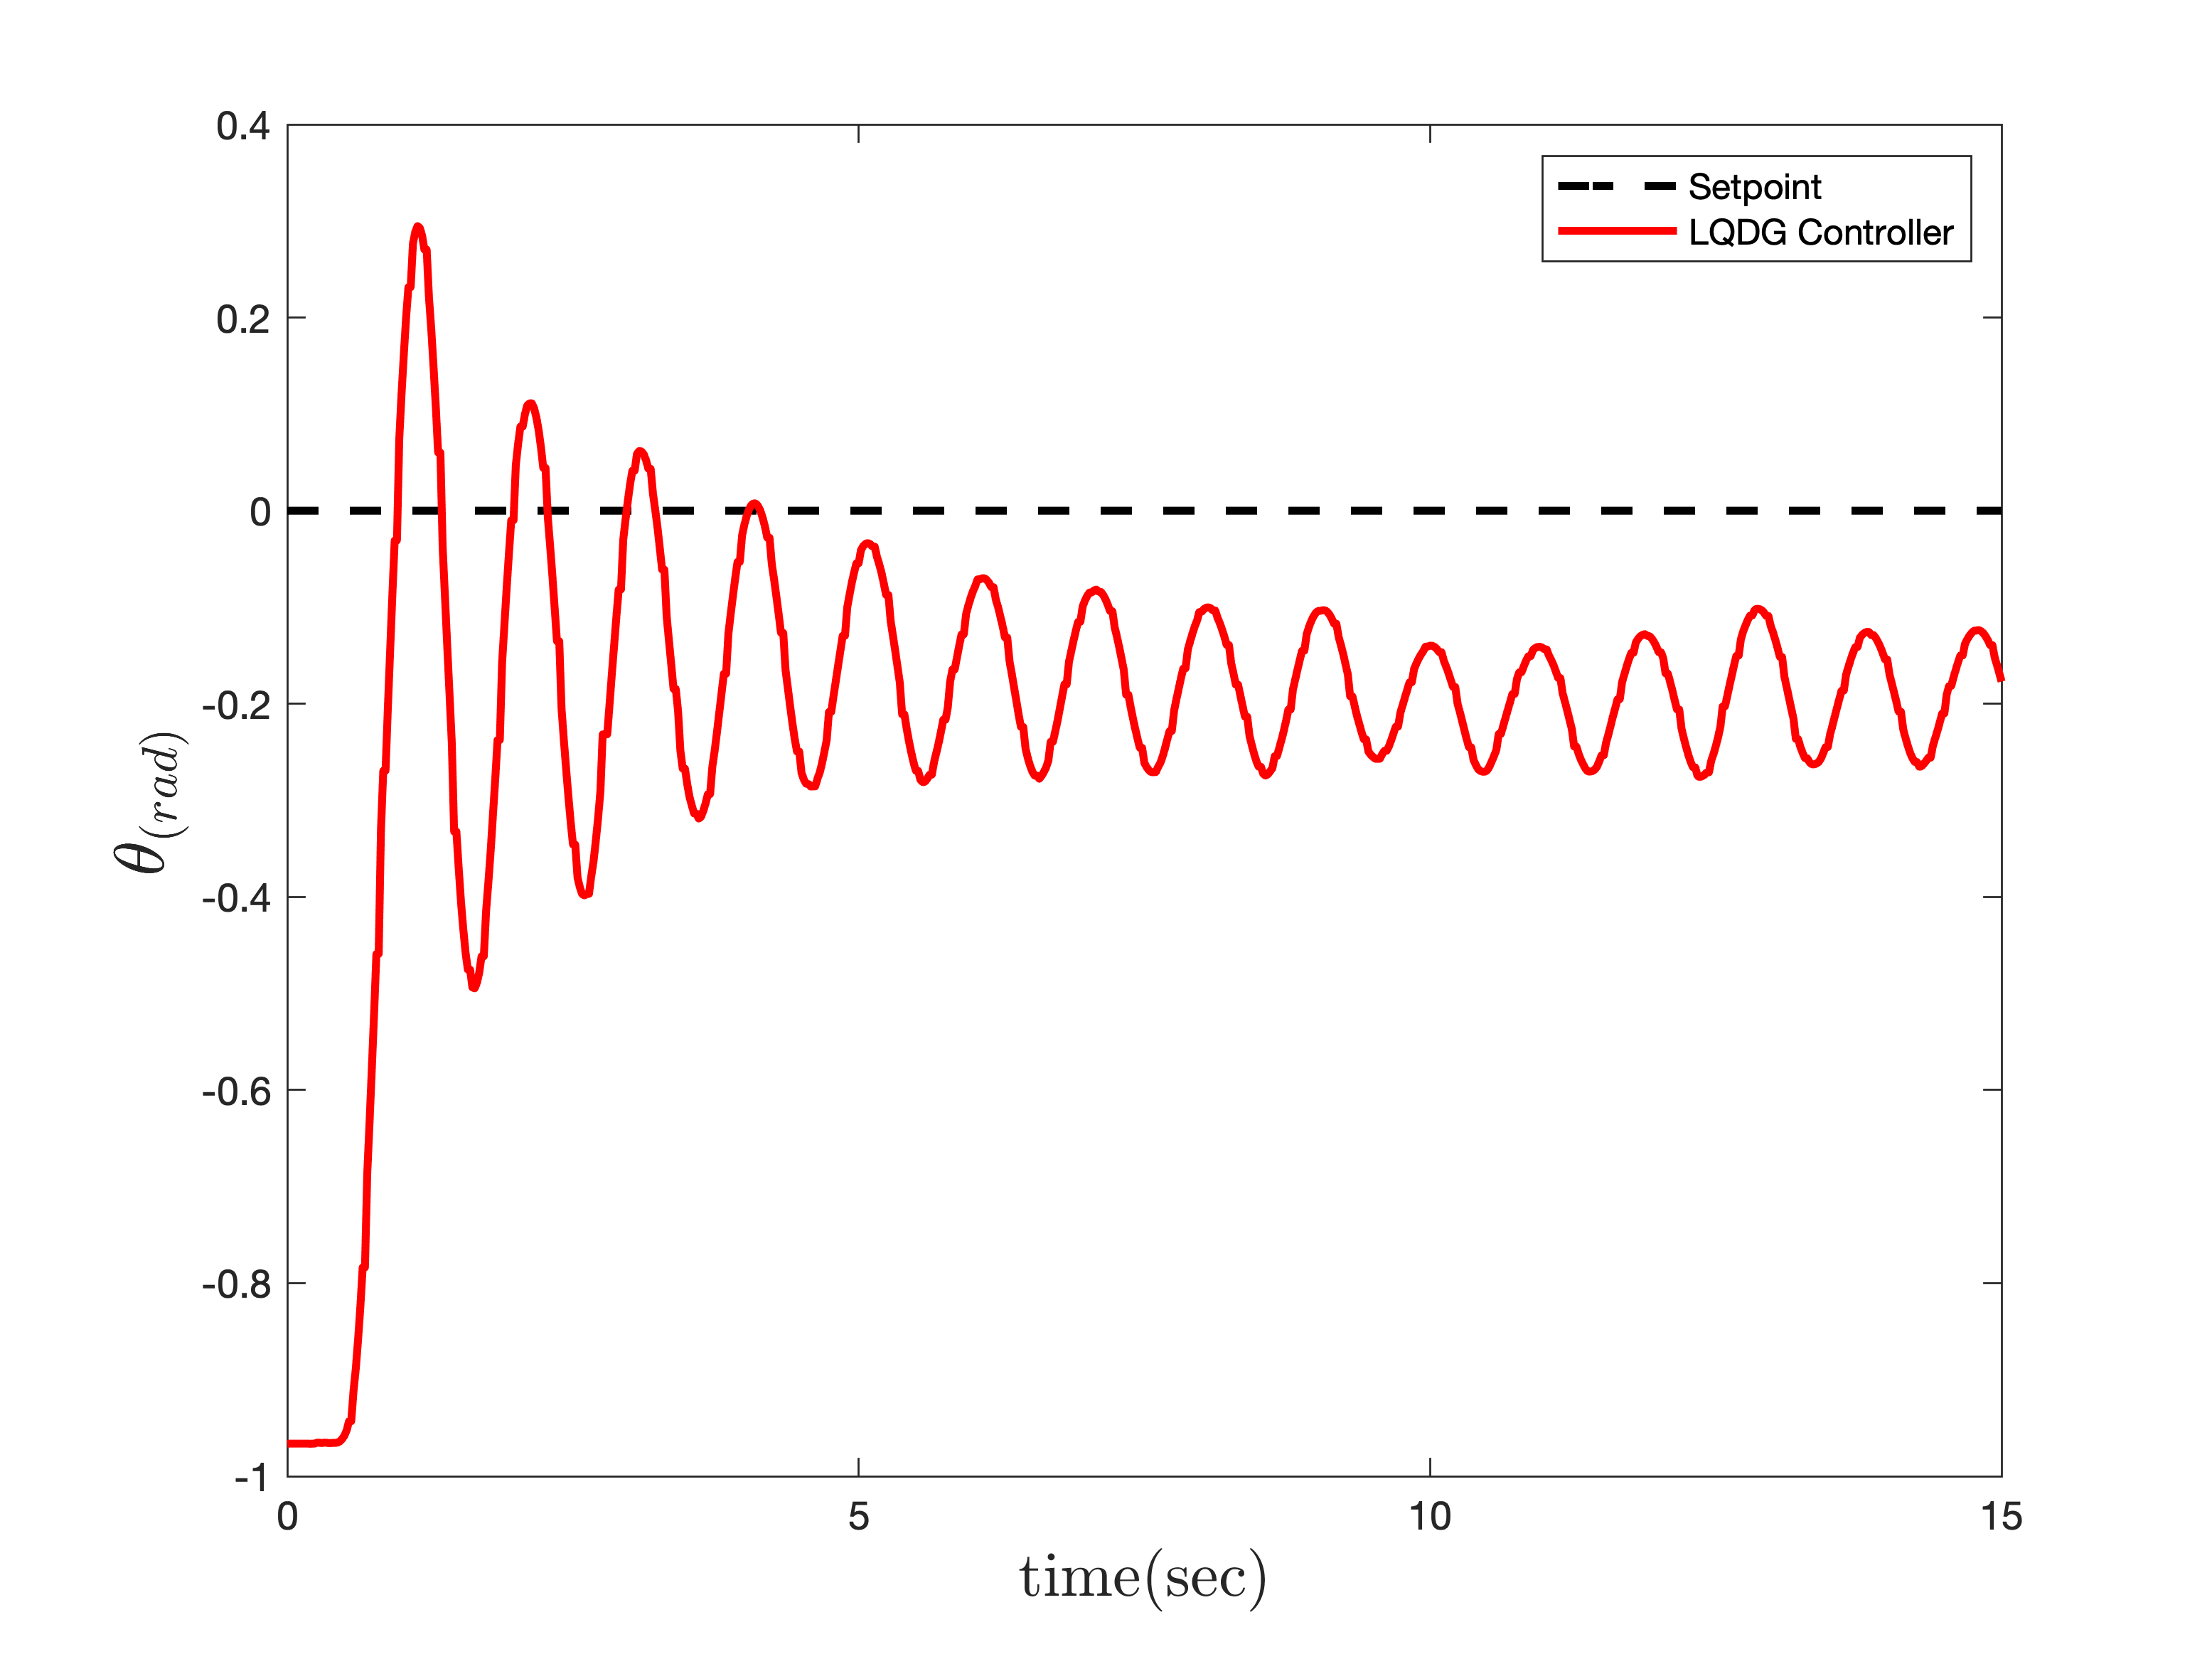
\includegraphics[width=.55\linewidth]{../Figures/Calibration/LQDG/Pitch/lqdg_pitch.png}
	\centering
	\caption{عملكرد LQDG در کنترل زاويه رول (تعقیب ورودی صفر)}
\end{figure}

\begin{figure}[H]
	\centering
	\subfigure[موتور شماره یک]{
		\centering
		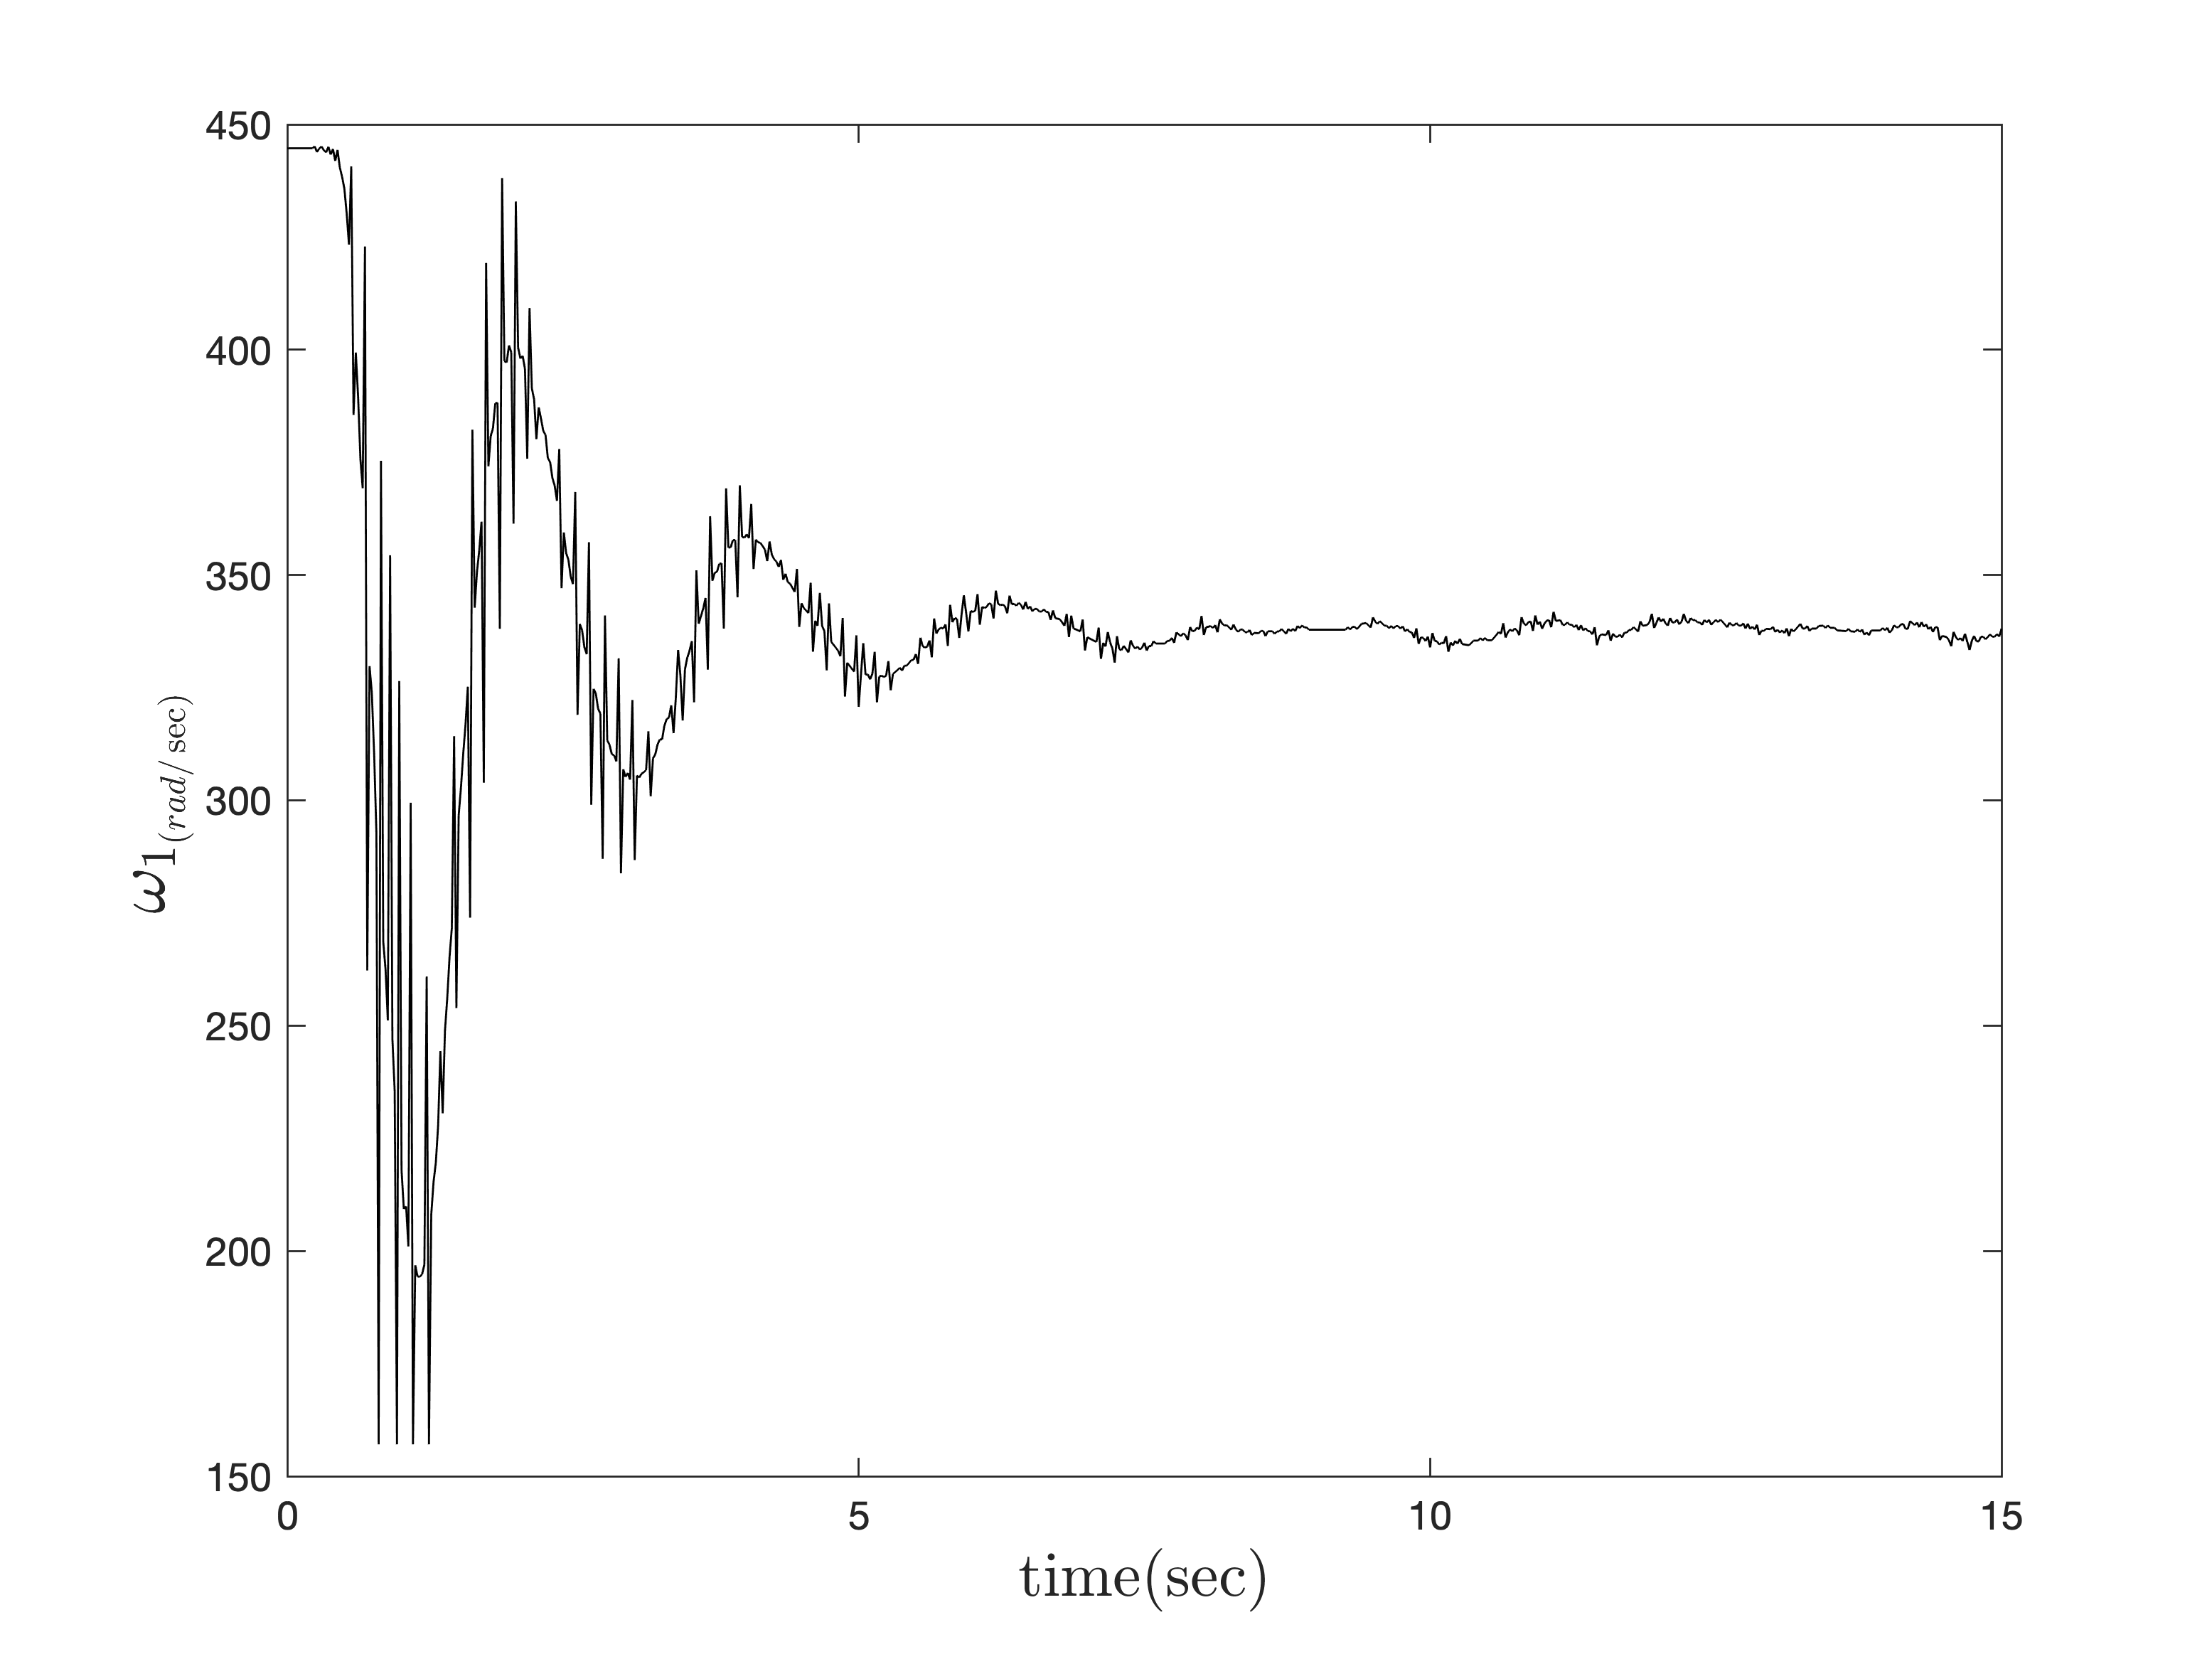
\includegraphics[width=.45\linewidth]{../Figures/Calibration/LQDG/Pitch/lqdg_pitch_Omega_1.png}
	}
	\subfigure[موتور شماره سه]{
		\centering
		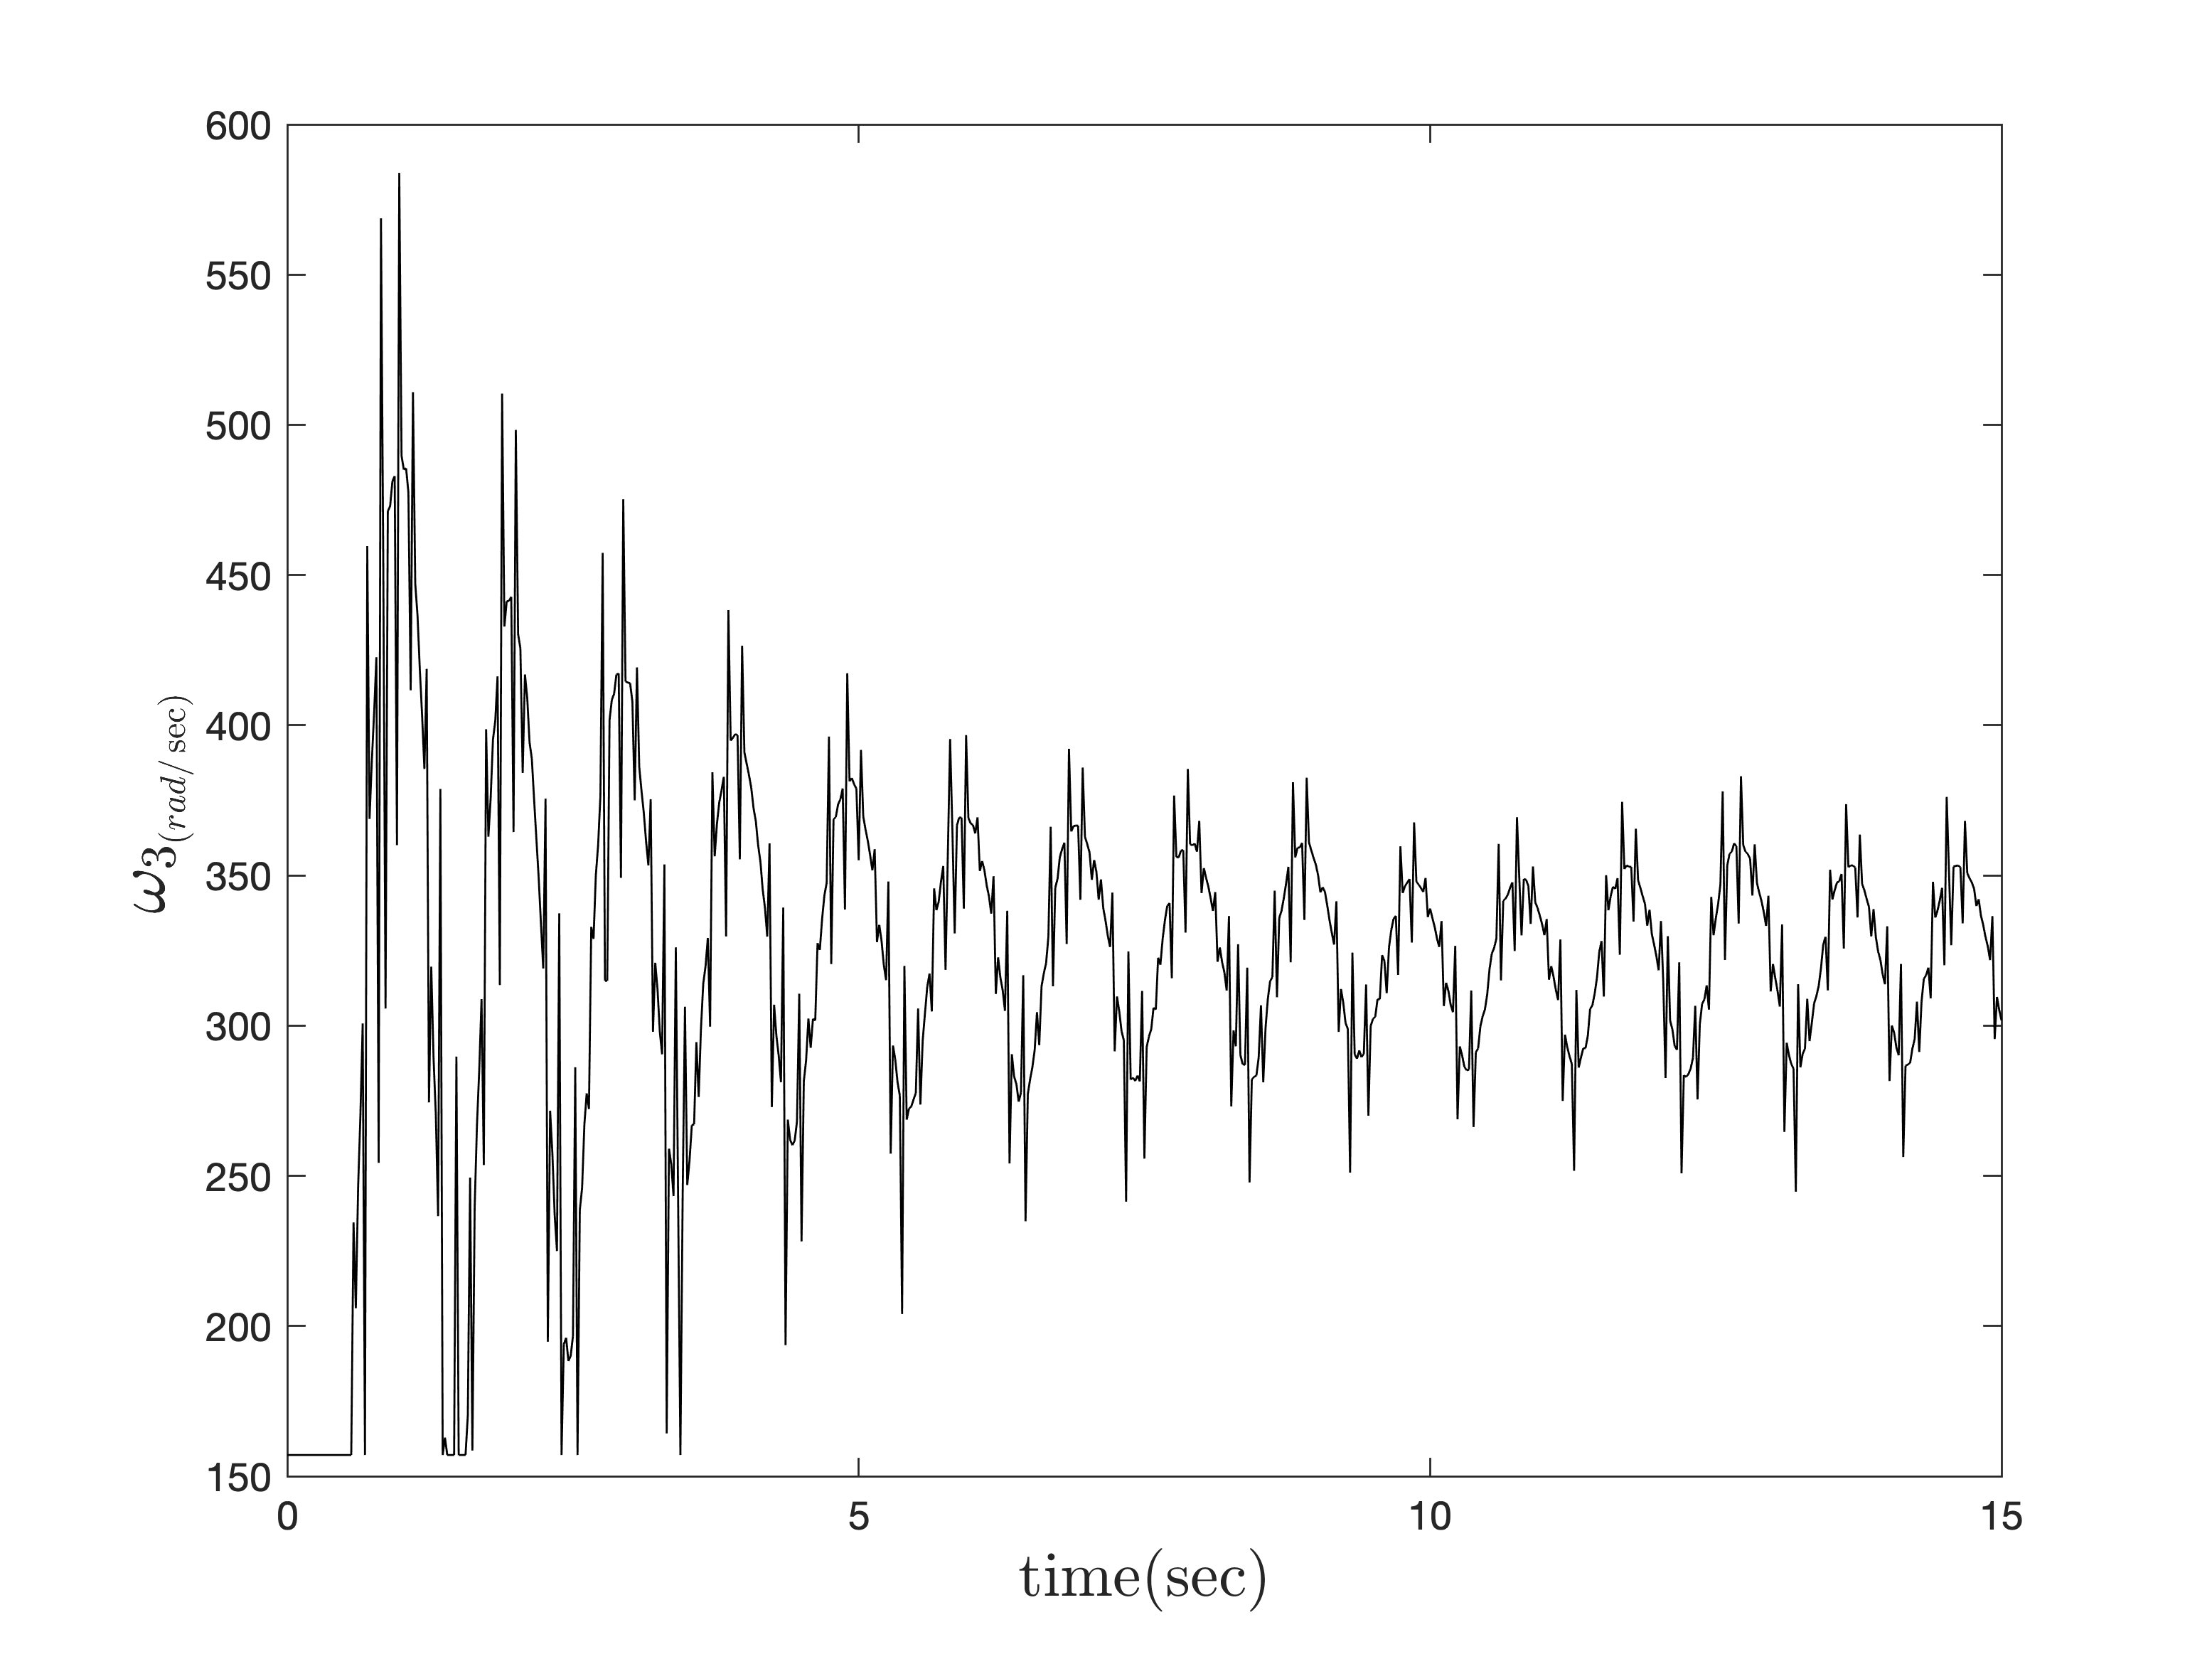
\includegraphics[width=.45\linewidth]{../Figures/Calibration/LQDG/Pitch/lqdg_pitch_Omega_3.png}
	}
	\caption{‫‪فرمان کنترلی موتورها در کنترل زاویه پیچ (تعقیب ورودی صفر)}
\end{figure}


بر اساس خروجی شبیه‌سازی (شکل
\ref{lqdg_roll_fig})
،کانال رول در حضور کنترل‌کننده LQDG در کمتر از پنج ثانیه به تعادل می‌رسد اما دارای خطای ماندگار است ولی خطای مانگار آن نسبت به کنترل‌کننده بخش
\ref{roll_lqr_section}
کمتر است. به دلیل خطای ماندگار، در بخش
%LQIDG
انتگرال‌گیر به کنترل‌کننده اضافه می‌شود تا خطای مانگار استند را کم کند.
